% ju 26-Dez-22
\documentclass[a4paper,12pt,fleqn,parskip=half]{scrartcl}
\usepackage[ngerman]{babel}
\usepackage[utf8]{inputenc}
\usepackage[T1]{fontenc}

% Schrift
%\usepackage{lmodern}
\usepackage[osf,sc]{mathpazo} 
\usepackage[scale=.9,semibold]{sourcecodepro}   
\usepackage[osf]{sourcesanspro}  

\usepackage[headsepline]{scrlayer-scrpage}
\pagestyle{scrheadings}
\clearpairofpagestyles

\usepackage[table,dvipsnames,usenames]{xcolor}
\usepackage{textcase}
\usepackage{nameref}
\usepackage{hyperref}
\usepackage{tabularx}
\usepackage{multirow}
\usepackage{multicol}
\usepackage{caption, booktabs}
\usepackage{graphicx} 
\usepackage{scrhack}    
\usepackage{url}%% Links
\usepackage[inline]{enumitem}
\usepackage{pifont}
\usepackage{eurosym}% \euro 20,-
\usepackage{amsmath}
\usepackage{amsfonts}
\usepackage{amssymb}
\usepackage{array}            % Extending the array and tabular environments
\usepackage{chngcntr}         % Change the resetting of counters
\usepackage[version=4]{mhchem}
\usepackage{stmaryrd}
\usepackage{siunitx}
\usepackage{float}
\usepackage{csquotes}
\usepackage{subcaption}
\usepackage{mathtools}
\usepackage{icomma}%Dezimaltrennzeichen
\usepackage{multimedia}%Video: \movie[externalviewer]{(video.mov)}{video.mov}
\usepackage{epstopdf}
\usepackage{footnote}
\usepackage{qrcode}% Anwendung: \qrcode[hyperlink,level=Q,version=2,height=1cm]{\website}
\usepackage{underscore}% Unterstrich ____

% PDF Dokumente einbinden
\usepackage{pdfpages}% \includepdf[pages=-]{Tabellen/Excel.pdf}
\RequirePackage{lastpage}  % Pagecounter

\addto\captionsngerman{%
\renewcommand{\figurename}{Abb.}
\renewcommand{\tablename}{Tab.}
}

% listings
\usepackage{listings}
\lstset{basicstyle=\linespread{1}\ttfamily\small,floatplacement=!htb,captionpos=t,abovecaptionskip=.5\baselineskip,belowcaptionskip=.5\baselineskip,upquote=true,showstringspaces=false,inputencoding=utf8,tabsize=4,
    	keywordstyle=\bfseries ,
	commentstyle=\color{rot5},
	stringstyle=\color{orange},
	breaklines=true,
  	postbreak=\mbox{\textcolor{black}{$\hookrightarrow$}\space},
	breakatwhitespace=false
}
\lstset{literate={á}{{\'a}}1 {é}{{\'e}}1 {í}{{\'i}}1 {ó}{{\'o}}1 {ú}{{\'u}}1 {Á}{{\'A}}1 {É}{{\'E}}1 {Í}{{\'I}}1 {Ó}{{\'O}}1 {Ú}{{\'U}}1 {à}{{\`a}}1 {è}{{\`e}}1 {ì}{{\`i}}1 {ò}{{\`o}}1 {ù}{{\`u}}1 {À}{{\`A}}1 {È}{{\'E}}1 {Ì}{{\`I}}1 {Ò}{{\`O}}1 {Ù}{{\`U}}1 {ä}{{\"a}}1 {ë}{{\"e}}1 {ï}{{\"i}}1 {ö}{{\"o}}1 {ü}{{\"u}}1 {Ä}{{\"A}}1 {Ë}{{\"E}}1 {Ï}{{\"I}}1 {Ö}{{\"O}}1 {Ü}{{\"U}}1 {â}{{\^a}}1 {ê}{{\^e}}1 {î}{{\^i}}1 {ô}{{\^o}}1 {û}{{\^u}}1 {Â}{{\^A}}1 {Ê}{{\^E}}1 {Î}{{\^I}}1 {Ô}{{\^O}}1 {Û}{{\^U}}1 {œ}{{\oe}}1 {Œ}{{\OE}}1 {æ}{{\ae}}1 {Æ}{{\AE}}1 {ß}{{\ss}}1 {ű}{{\H{u}}}1 {Ű}{{\H{U}}}1 {ő}{{\H{o}}}1 {Ő}{{\H{O}}}1 {ç}{{\c c}}1 {Ç}{{\c C}}1 {ø}{{\o}}1 {å}{{\r a}}1 {Å}{{\r A}}1 {€}{{\EUR}}1 {£}{{\pounds}}1 {~}{{\textasciitilde}}1 {-}{{-}}1 }

% bibliography
\usepackage[
    bibencoding=utf8,
    backend=biber,% bibtex, biber
    backref=false,backrefstyle=three+,url=true,urldate=comp,abbreviate=false,maxnames=20
]{biblatex} %Paket laden
\DeclareBibliographyCategory{cited}
\let\defaultcite\cite\renewcommand*\cite[2][]{\addtocategory{cited}{#2}\defaultcite[#1]{#2}}
\let\defaulttextcite\textcite\renewcommand*\textcite[2][]{\addtocategory{cited}{#2}\defaulttextcite[#1]{#2}}
\setcounter{biburllcpenalty}{7000}
\setcounter{biburlucpenalty}{8000}
\AfterPackage{biblatex}{
	\PreventPackageFromLoading[\errmessage{Sie haben versucht, das Cite-Paket zu laden, das nicht mit biblatex kompatibel ist.}]{cite}
}

\hypersetup{%
	%pdftitle={\titel},
	%pdfsubject={Latex},
	%pdfauthor={\autor},
	%pdfcreator={\autor}, 
	bookmarksnumbered=true,
	breaklinks=true,
	%colorlinks=true,	   
	linkcolor=rot5,		
	filecolor=blau5,		
	urlcolor=blau5,			
	citecolor=ForestGreen
}

\linespread{1.1}
\setlist{itemsep=0pt}
\widowpenalty10000
\clubpenalty10000
\tolerance1000   

\usepackage[left=2cm,right=2cm,top=1cm,bottom=1cm,includeheadfoot]{geometry}
%\usepackage[left=4cm,right=2cm,top=1cm, bottom=1cm,includeheadfoot]{geometry}
%\usepackage[left=6cm,right=1cm,top=1cm, bottom=1cm,includeheadfoot]{geometry}
%\usepackage[landscape=true,left=2cm,right=2cm,top=1cm,bottom=1cm,includeheadfoot]{geometry}%quer

% eigene Farbe definieren
% Adobe Prozessfarben: CMYK: 100,50,0,35 -> 1,0.5,0,0.35
\definecolor{orange}{cmyk}{0,0.55,0.61,0}   % 0,55,61,0
\definecolor{blau5}{cmyk}{1,0.77,0.1,0.01}  % 100,77,10,
\definecolor{rot5}{cmyk}{0.22,1,1,0.19}     % 22,100,100,19
\definecolor{grau2}{cmyk}{0,0,0,0.1}        % 0,0,0,40
\definecolor{blau}{cmyk}{0.93,0.66,0,0.21}% 

% Literatur
\bibliography{content/literatur}
\bibliography{content/literatur-kfz}
\bibliography{content/literatur-sport}

%%%%%%%%%%%%%%%%%%%%%%%%%%%%%%%%%%%%%%%%%%%%%%%%%%%%%%%
\newcommand{\name}{Jan Unger}
\newcommand{\thema}{EDC-Elektronische-Dieselsteuerung}
\newcommand{\quelle}{\name}
\newcommand{\website}{https://bw-ju.de/}
\newcommand{\github}{https://github.com/ju1-eu}
%%%%%%%%%%%%%%%%%%%%%%%%%%%%%%%%%%%%%%%%%%%%%%%%%%%%%%%

\ihead{\textbf{Quelle:} \quelle}%{Kopfzeile innen}
\ohead{\textbf{Datum:} \today}  %{Kopfzeile außen}
\ifoot{\textbf{Thema:} \thema}  %{Fußzeile  innen}
\ofoot{Seite {\thepage} von {\pageref{LastPage}}}%{Fußzeile  außen}

\title{\thema}
\author{\name}
\date{\today}

\begin{document}
	%%%%%%%%%%%%%%%%%%%%%%%%%%%%%%%%%%%%%%%%%%%%%%%%%%%%%%%%%%%%%%%%%%
	\begin{abstract}
		\center
		\textbf{\Large \thema}%14pt
		
		\vspace{1.5em}
		%\datum	
		%\qrcode[hyperlink,level=Q,version=2,height=1cm]{\website}
		\qrcode[hyperlink,level=Q,version=2,height=1cm]{\github}
		
		\vspace{1.5em} 
		\raggedright
		\textbf{\large Keywords}
		% Checkliste
		\begin{itemize}[label=\checkmark]
			\item Begriff
		\end{itemize}
	\end{abstract}
    %%%%%%%%%%%%%%%%%%%%%%%%%%%%%%%%%%%%%%%%%%%%%%%%%%%%%%%%%%%%%%%%%%

	% anpassen
	%\input{content/tex/neu}
	%ju 31-Dez-22 EDC-Elektronische-Dieselsteuerung.tex
\section{Aufgaben der
Motorsteuerung}\label{aufgaben-der-motorsteuerung}

\begin{enumerate}
\item
  Einspritzung des Kraftstoffes in die Zylinder
\item
  Regelung und Begrenzung von Drehzahl und Geschwindigkeit,
\item
  Regelung des Luftsystems (Abgasrückführung und Ladedruckregelung),
\item
  Abgasnachbehandlung,
\item
  Glühkerzensteuerung und Thermomanagement,
\item
  Zylinderabschaltung,
\item
  Diagnose,
\item
  Wegfahrsperre.
\end{enumerate}

\newpage

\section{Einspritzung}\label{einspritzung}

Quelle: S. 57 \textcite{borgeest:2021:elektronik}.

\begin{figure}[!ht]% hier: !ht
\centering
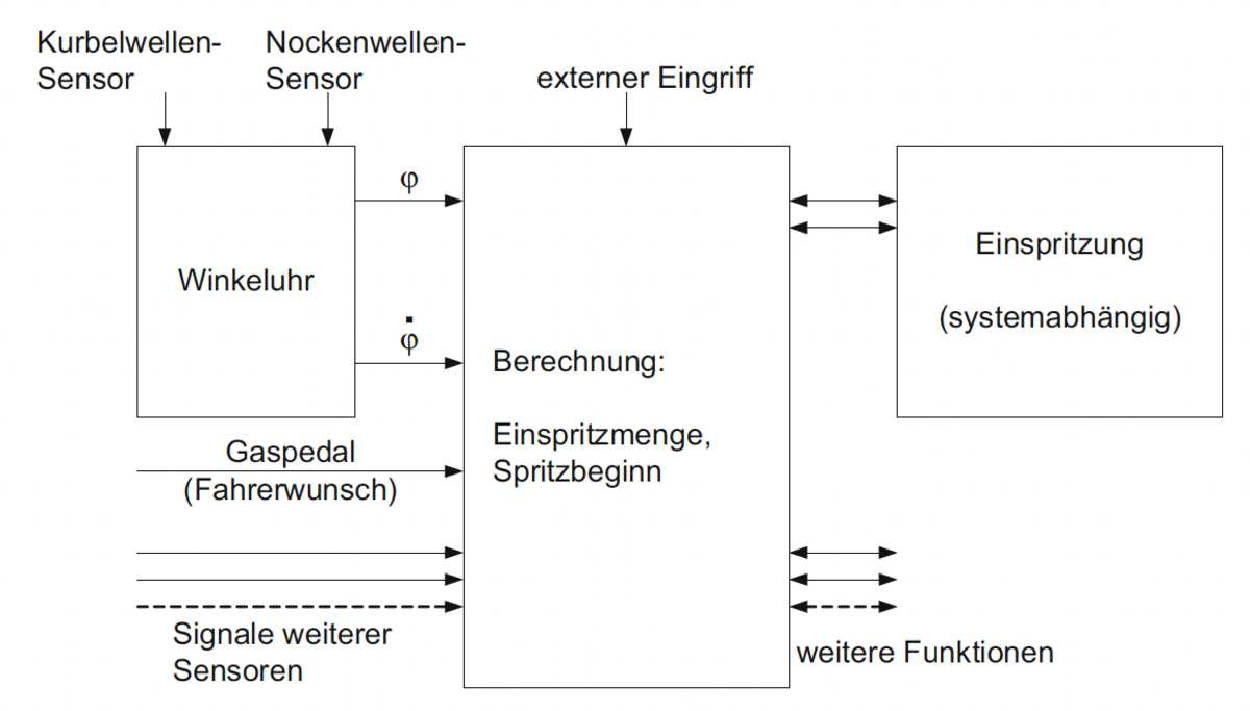
\includegraphics[width=0.7\textwidth]{images/EDC/EDC-1.pdf}
\caption{Einspritzfunktion eines Dieselsteuergerätes ($\varphi$:
Kurbelwellenwinkel). (Bild: Kai Borgeest)}
%\label{fig:}%% anpassen
\end{figure}

\begin{itemize}
\item
  SG optimalen Zeitpunkt für den Beginn der Einspritzung berechnet und
  die >>richtige<< Menge für die Einspritzung kennt.

  \begin{itemize}
  \item
    Einspritzmenge
  \item
    Zeitpunkt / Spritzbeginn
  \end{itemize}
\item
  Ansteuern der Einspritzventile für jeden Zylinder
\item
  Fahrpedal (Fahrerwunsch)
\item
  Winkeluhr im SG

  \begin{itemize}
  \item
    aktuelle Stellung der Kurbelwelle und Drehzahl
  \item
    zeitlich veränderliche Vorgänge im Motor nicht direkt als Funktion
    der Zeit, sondern als Funktion des Kurbelwellenwinkels
    (winkelsynchron) anzugeben und zu berechnen
  \item
    In der Zeit $\Delta t$ bewegt sich bei der Drehzahl $n$ die
    Kurbelwelle um den Winkel
  \item
    $\Delta \varphi = 6 \cdot n \cdot \Delta t$
    $\quad [^\circ \text{KW} = \text{min}^{-1} \cdot \text{s}]$
  \end{itemize}
\item
  Einspritzung bei

  \begin{itemize}
  \item
    $0^\circ$ bedeutet das der Kolben bei einem als Bezug gewählten
    Zylinder gerade am oberen Totpunkt steht.
  \item
    $-10^\circ$ bedeuten, dass sich die Kurbelwelle noch um
    $10^\circ$ drehen muss, bis der Kolben im Bezugszylinder den OT
    erreicht hat.
  \item
    $+10^\circ$ bedeuten, dass der Kolben schon wieder auf dem Weg vom
    OT nach unten ist.
  \end{itemize}
\end{itemize}

\newpage

\begin{figure}[!ht]% hier: !ht
\centering
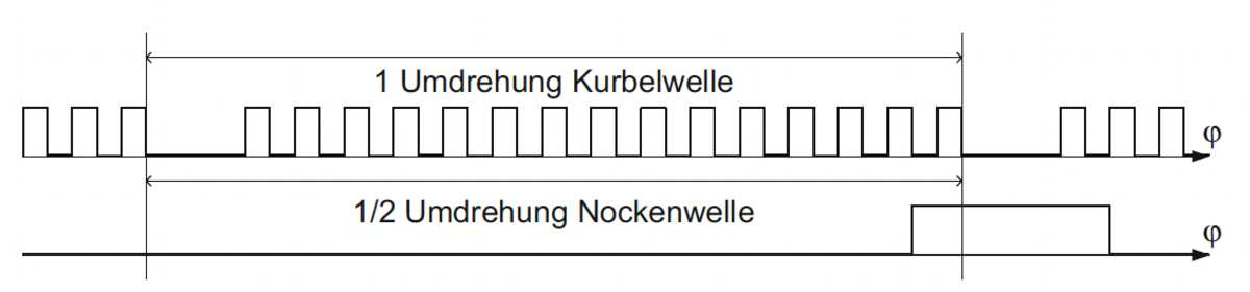
\includegraphics[width=0.5\textwidth]{images/EDC/EDC-3.pdf}
\caption{Signale vom Kurbelwellen- und Nockenwellensensor. (Bild: Kai
Borgeest)}
%\label{fig:}%% anpassen
\end{figure}

\textbf{Kurbelwellensensor}

\begin{itemize}
\item
  Impulsgeber, dessen Impulsfrequenz steigt mit der Drehzahl. Durch
  abzählen der Impulse lässt sich der Winkel bestimmen.
\end{itemize}

\textbf{Nockenwellensensor}

\begin{itemize}
\item
  OT-Verbrennung (Bezugsmarke/Referenzmarke) in $^\circ \text{KW}$
\end{itemize}

\begin{figure}[!ht]% hier: !ht
\centering
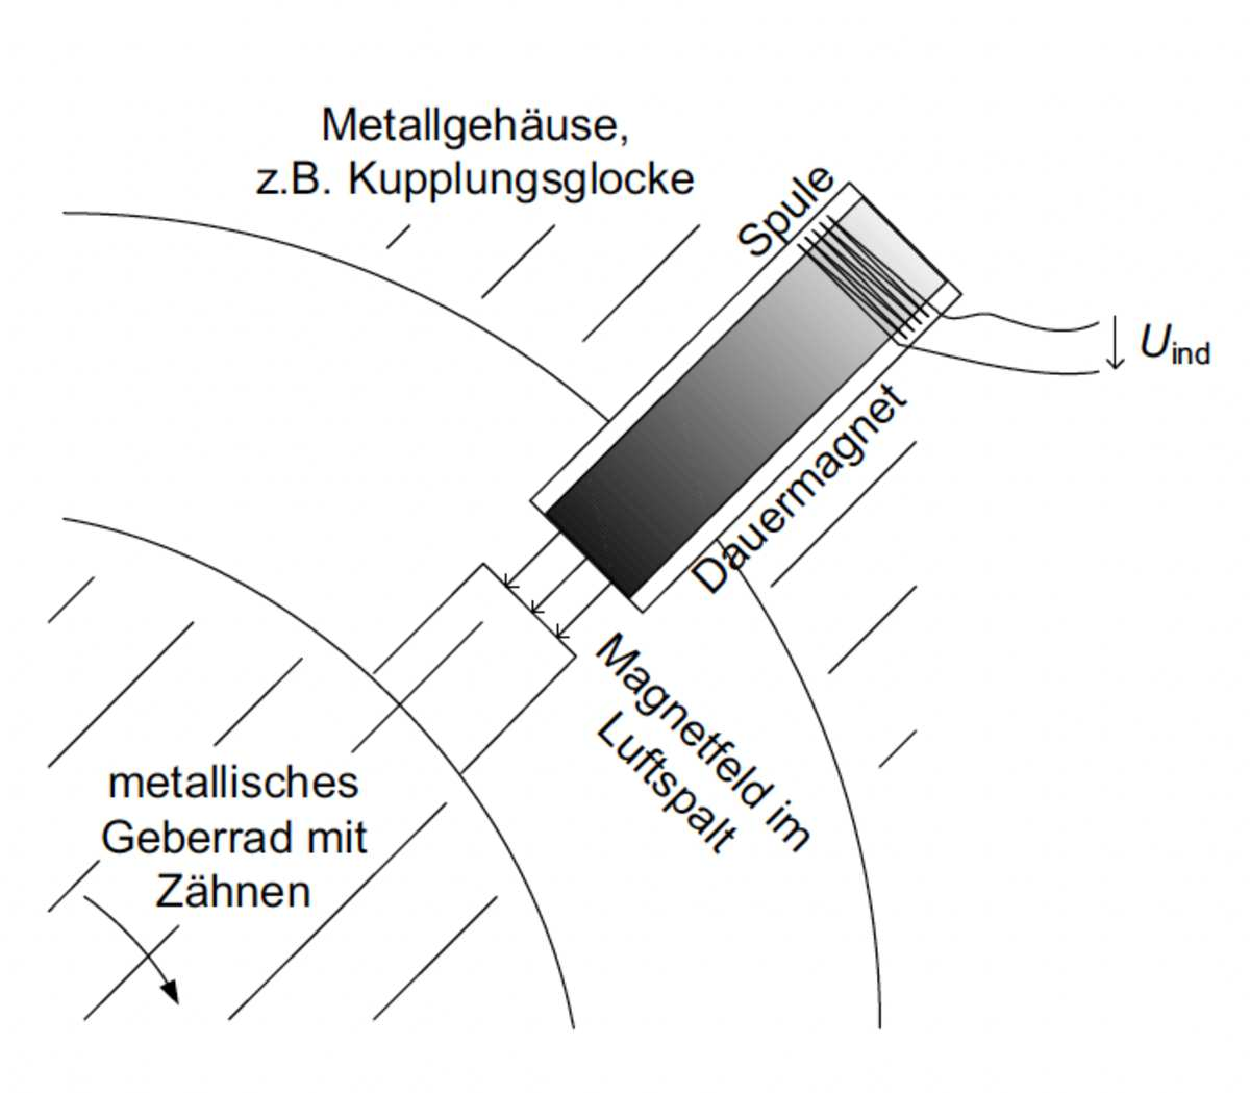
\includegraphics[width=0.3\textwidth]{images/EDC/EDC-4.pdf}
\caption{Elektromagnetischer Sensor für die Drehzahl der Kurbelwelle.
Die nur im Luftspalt eingezeichneten Magnetfeldlinien schließen sich
über das Zahnrad, dessen Lagerung und über das Gehäuse, welches das
Zahnrad umfasst und den Sensor aufnimmt. Durch Änderung des Feldes wird
in der Spule die Spannung $U_{\text{ind}}$ induziert. (Bild: Kai
Borgeest)}
%\label{fig:}%% anpassen
\end{figure}

\newpage

\textbf{4-Zylinder Motor:}

\begin{itemize}
\item
  $0^\circ (\text{Kolben im OT, Einspritzung Verbrennung}), 180^\circ (\text{UT})$
\item
  und
  $360^\circ (\text{Kolben im OT, Ausstoßen}), 540^\circ (\text{UT})$
\item
  zweideutigkeit (Kolben 2x im OT pro Arbeitsspiel)
\item
  alle 4x-Takte: Ansaugen, Verdichten, Arbeiten/Verbrennen, Ausstoßen
\item
  zwei Kurbelwellenumdrehungen ($720^\circ$), eine
  Nockenwellenumdrehung
\end{itemize}

\begin{figure}[!ht]% hier: !ht
\centering
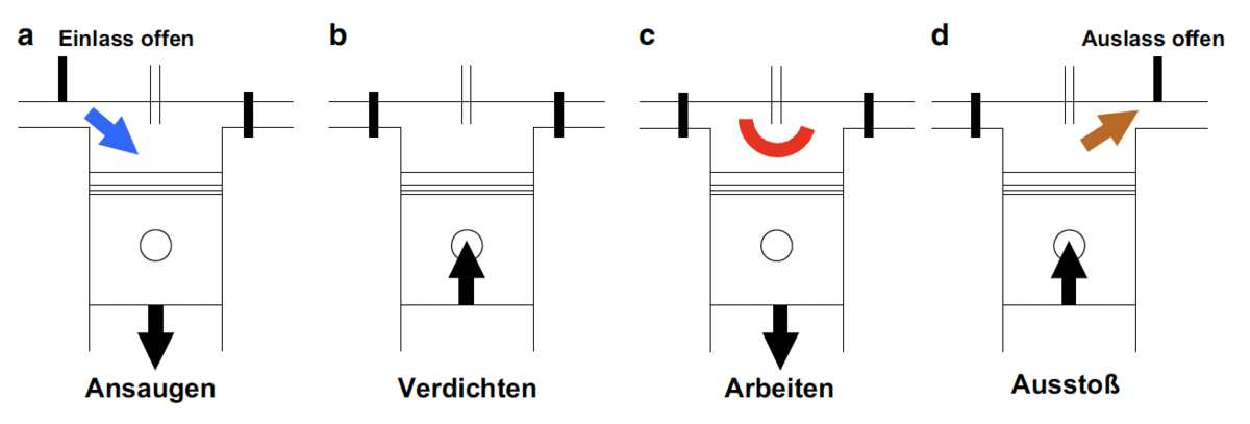
\includegraphics[width=0.7\textwidth]{images/EDC/EDC-2.pdf}
\caption{Darstellung der vier Takte eines Viertaktmotors von links nach
rechts: a Beginn des Ansaugtaktes ($360-540^\circ$): Bei geöffneten
Einlassventil saugt der sich abwärts bewegende Kolben Luft an. b Ende
des Verdichtungstaktes ($540-720^\circ$): Beide Ventile sind
geschlossen, durch die Aufwärtsbewegung des Kolbens wird die Luft
komprimiert und dadurch erhitzt. c Beginn des Arbeitstaktes
($0-180^\circ$): Der Kraftstoff wird eingespritzt und verbrennt durch
die hohe Lufttemperatur. Dadurch wird der Kolben nach unten gedrückt. d
Ende des Ausstoßtaktes ($180-360^\circ$): Durch das nun geöffnete
Auslassventil drückt der wieder steigende Kolben die Verbrennungsgase
aus dem Zylinder heraus. (Bild: Kai Borgeest)}
%\label{fig:}%% anpassen
\end{figure}

\newpage

\subsection{Berechnung der
Einspritzmenge}\label{berechnung-der-einspritzmenge}

\textbf{Fahrzustände}

\begin{itemize}
\item
  Start, Leerlauf, Fahren
\item
  \textbf{Schubbetrieb} bei Bergabfahrt mit einem niedrigen Gang; in
  diesem Falle bremst der Motor das bergab rollende Fahrzeug.
\item
  \textbf{Teillast und Volllast}
\item
  \textbf{Notlauf} Steuergerät erkennt einen kritischen Zustand oder
\item
  \textbf{Grenzzustände} (z. B. das Abregeln bei Erreichen von Drehzahl-
  oder Geschwindigkeitsgrenzen).
\end{itemize}

Die \textbf{Einspritzmenge} berechnet sich über einen weiten Bereich
näherungsweise proportional aus dem angeforderten Drehmoment
(Fahrerwunsch), bzw. im Leerlauf von der Anforderung des
Leerlaufreglers.

Fahrerwunsch wird vom Gaspedal über einen Pedalwertgeber (PWG, Sensor
der einen Winkel in eine Spannung umsetzt) elektrisch an das Steuergerät
übertragen.

\textbf{weitere Parameter für das Drehmoment bzw. die Einspritzmenge}

\begin{itemize}
\item
  aktuelle Drehzahl
\item
  aktuelle Fahrgeschwindigkeit
\item
  Motorlast
\item
  Temperatur des Motors (gemessen über die Kühlwassertemperatur,
  Öltemperatur),
\item
  Batteriespannung
\item
  Informationen über das Getriebe
\item
  Betriebszustand (z. B. Kaltstart)
\item
  Begrenzungen (z. B. Rauchbegrenzung)
\end{itemize}

\textbf{Mengenberechnung}

\begin{enumerate}
\item
  \textbf{Mengenpfad} oder

  \begin{itemize}
  \item
    berechnet grob die erforderliche Einspritzmenge, passt diese dann
    durch etliche Korrekturrechnungen, Kennfelder, Begrenzungen und
    eventuelle externe Mengeneingriffe auf die exakt benötigte Menge an.
  \end{itemize}
\item
  \textbf{Momentenpfad}

  \begin{itemize}
  \item
    wird zuerst das vom Motor benötigte Drehmoment grob berechnet,
    sämtliche Berechnungen im Steuergerät werden mit Momenten statt mit
    Mengen durchgeführt und erst zum Schluss des Berechnungspfades wird
    die genaue Momentenanforderung in die exakte Einspritzmenge
    umgerechnet.
  \end{itemize}
\end{enumerate}

Bei externen Eingriffen (Signale von anderen Steuergeräten) kann die
Momentenstruktur als >>gemeinsame Sprache<< mehrerer Steuergeräte
vorteilhaft sein, da Getriebesteuergeräte und Fahrdynamiksteuergeräte
intern mit mechanischen Größen und nicht mit Kraftstoffmengen rechnen.

\begin{enumerate}
\item
  \textbf{Voreinspritzung} zur Geräuschminderung

  \begin{itemize}
  \item
    PKW in der Größenordnung von $1 - 2~mm^3$
  \end{itemize}
\item
  \textbf{Haupteinspritzung} Drehmoment

  \begin{itemize}
  \item
    PKW in der Größenordnung von einiger $10~mm^3$
  \end{itemize}
\item
  \textbf{Nacheinspritzung} zur Nachverbrennung von Partikeln im
  Zylinder oder zur Unterstützung der Abgasnachbehandlung.

  \begin{itemize}
  \item
    PKW in der Größenordnung von $1 - 2~mm^3$
  \end{itemize}
\end{enumerate}

Vgl. Wassertropfen ein Volumen von ca. $30~mm^3$

\newpage

\subsection{Berechnung des
Spritzbeginns}\label{berechnung-des-spritzbeginns}

\begin{enumerate}
\item
  \textbf{frühe Einspritzung} führt zu einer zu frühen Verbrennung.
  Dadurch wird bereits eine Kraft von oben auf den Kolben ausgeübt,
  bevor er den OT erreicht. Dies führt zu einem Verlust an Leistung, im
  Extremfall sogar zum Stillstand oder zur Beschädigung des Motors.
  Weiterhin erreicht die Verbrennungstemperatur zu hohe Spitzenwerte,
  die zu einer vermehrten Bildung von Stickoxiden im Abgas führen.
\item
  \textbf{späte Einspritzung} führt dazu, dass der eingespritzte
  Kraftstoff nicht mehr vollständig verbrennt. Dadurch geht ebenfalls
  Leistung verloren und es bildet sich schwarzer Rauch, der Partikel
  enthält. Bei noch späterer Einspritzung wird der Kraftstoff völlig
  unverbrannt ausgestoßen, das Abgas färbt sich bläulich und riecht nach
  Diesel. Im Extremfall, wenn unverbrannter Kraftstoff sich als
  Flüssigkeit in der Kolbenmulde ansammelt, kommt es zum Motorschaden.
\end{enumerate}

Bereits bei einer Abweichung des Spritzbeginns um $1^\circ \text{KW}$
lassen sich die gültigen Abgasgrenzwerte nicht mehr einhalten.

Der \textbf{optimale Spritzbeginn} ist keine Konstante, sondern er hängt
vom Motor und von mehreren Betriebsparametern ab. (leistungsoptimierte,
abgasoptimierte Spritzbeginn)

\textbf{Parameter}

\begin{itemize}
\item
  Drehzahl und die Einspritzmenge

  \begin{itemize}
  \item
    Sowohl mit steigender Drehzahl als auch mit zunehmender Menge wird
    der Spritzbeginn nach früh verschoben.
  \end{itemize}
\item
  Temperatur des Motors
\item
  Temperatur der Ansaugluft
\item
  atmosphärische Druck.
\end{itemize}

Im Steuergerät wird der Zusammenhang zwischen den gemessenen Parametern
und dem daraus ermittelten Spritzbeginn durch Formeln oder über
Kennlinien und Kennfelder, also über Wertetabellen dargestellt. Diese
werden zunächst mit Erfahrungswerten gefüllt, dann erfolgt am Prüfstand
eine experimentelle Optimierung.

\newpage

\subsection{Ansteuerung des
Einspritzsystems}\label{ansteuerung-des-einspritzsystems}

\begin{figure}[!ht]% hier: !ht
\centering
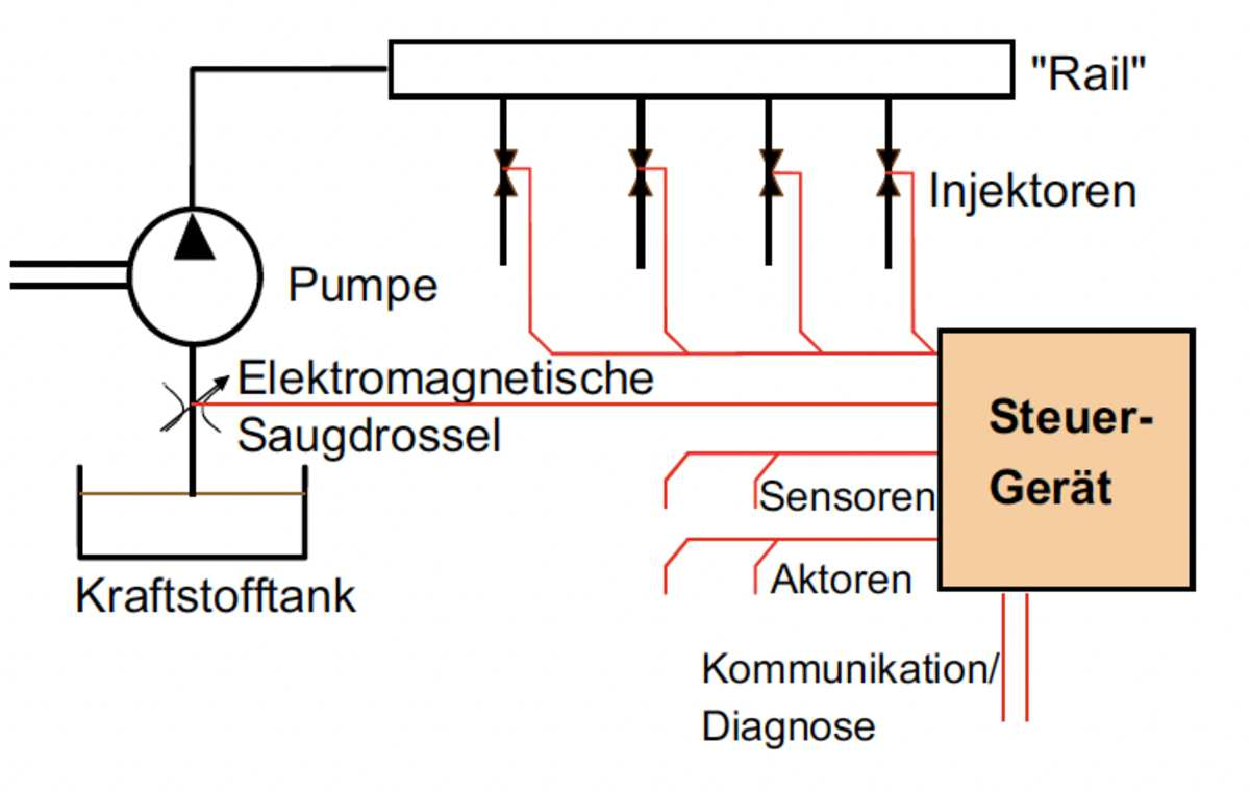
\includegraphics[width=0.5\textwidth]{images/EDC/EDC-5.pdf}
\caption{Überblick über ein Common-Rail-Einspritzsystem. (Bild: Kai
Borgeest)}
%\label{fig:}%% anpassen
\end{figure}

\textbf{Common-Rail-System}

\textbf{Vorteil von Common Rail} ist, dass permanent Kraftstoff
einspritzbereit unter einem hohen, über mehrere Einspritzungen konstant
regelbaren Druck verfügbar ist.

\textbf{Nachteil von älteren Einspritzsystemen} (Reihenpumpen,
Einzelpumpen, Verteilerpumpen, Pumpe-Düse, Pumpe-Leitung-Düse) Druck ist
nur zu bestimmten Zeiten, in denen ein Nocken einen Pumpenkolben
betätigt verfügbar.

\begin{itemize}
\item
  \textbf{Rail} rohrförmiger Druckbehälter mit Kraftstoff
\item
  Über kurze Leitungen ist je ein Injektor (Einspritzventil) pro
  Zylinder mit dem Rail verbunden.
\item
  Der Injektor kann vom Steuergerät (ECU) zu definierten Zeiten zur
  Einspritzung geöffnet werden.

  \begin{itemize}
  \item
    \textbf{Piezo-Injektoren} und \textbf{elektromagnetischen
    Injektoren}
  \end{itemize}
\item
  Die eingespritzte Menge hängt von der elektrischen Ansteuerdauer (die
  ungefähr der Dauer entspricht, in der der Injektor geöffnet ist) und
  vom Druck im Rail ab.
\item
  Den Druck im Rail bis 2700 bar, bei LKW bis 3000 bar, erzeugt eine
  Kolbenpumpe.
\item
  Aufgrund der Systemkosten, des Energieaufwandes und der
  Druckwellenproblematik in den Leitungen bei Drücken oberhalb 2000 bar
  arbeiten einige neue Systeme mit einem Raildruck unterhalb 1000 bar
  und erhöhen erst unmittelbar vor der Einspritzung, idealerweise erst
  im Injektor, den Druck über einen hydraulischen Übersetzerkolben auf
  den Einspritzdruck von z. B. 2500 bar.

  \begin{itemize}
  \item
    APCRS (Amplifier Piston Common Rail System) oder druckverstärktes
    Common Rail. Ein Pilotsystem ist das seit 2011 in LKW-Motoren
    eingesetzte >>X-Pulse<< - System von Daimler.
  \end{itemize}
\end{itemize}

\newpage

\subsection{Ansteuerung der
Injektoren}\label{ansteuerung-der-injektoren}

\begin{figure}[!ht]% hier: !ht
\centering
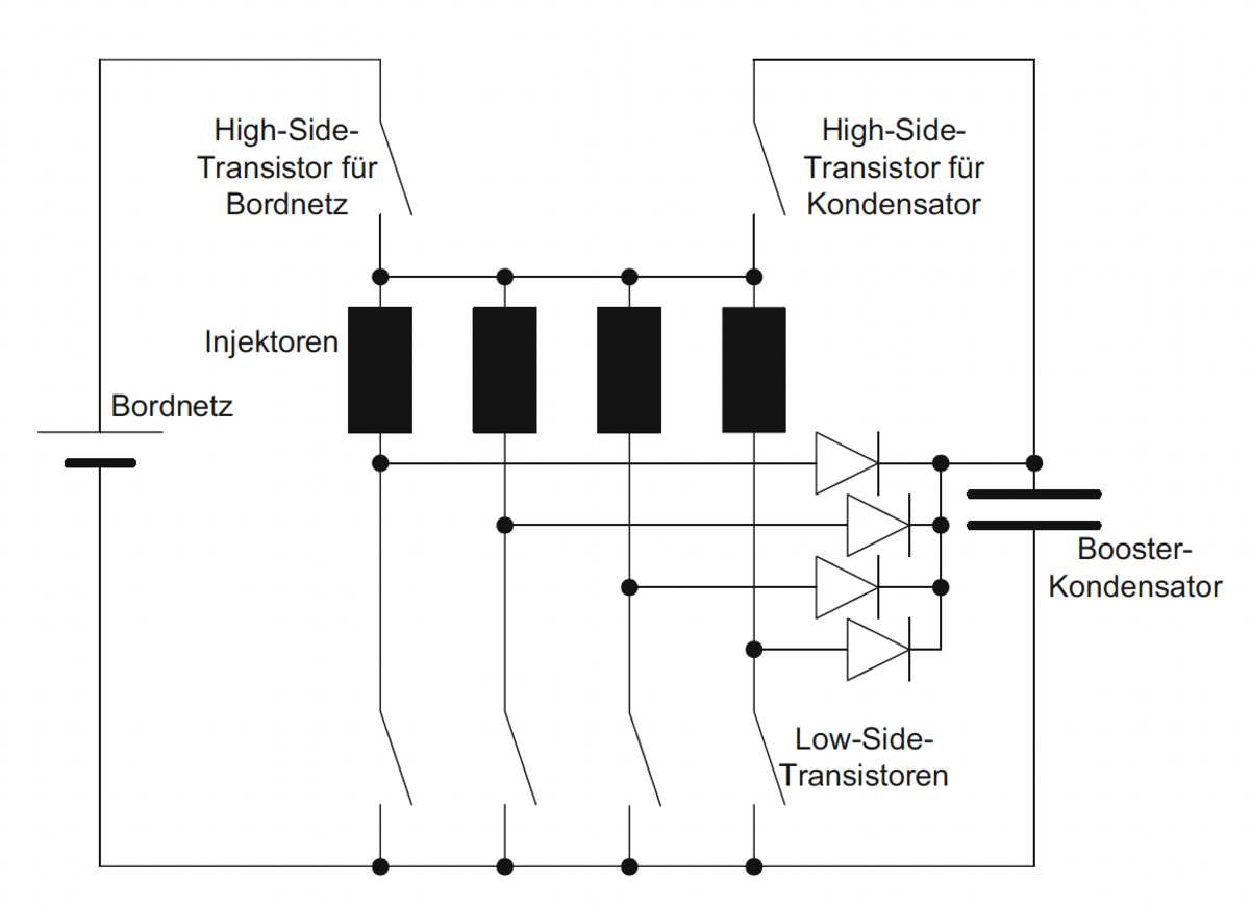
\includegraphics[width=0.5\textwidth]{images/EDC/EDC-8.pdf}
\caption{Ansteuerschaltung für Common-Rail-Injektoren mit Magnetventilen
(Prinzip). (Bild: Kai Borgeest)}
%\label{fig:}%% anpassen
\end{figure}

\textbf{Injektoren mit Magnetventil}

\begin{figure}[!ht]% hier: !ht
\centering
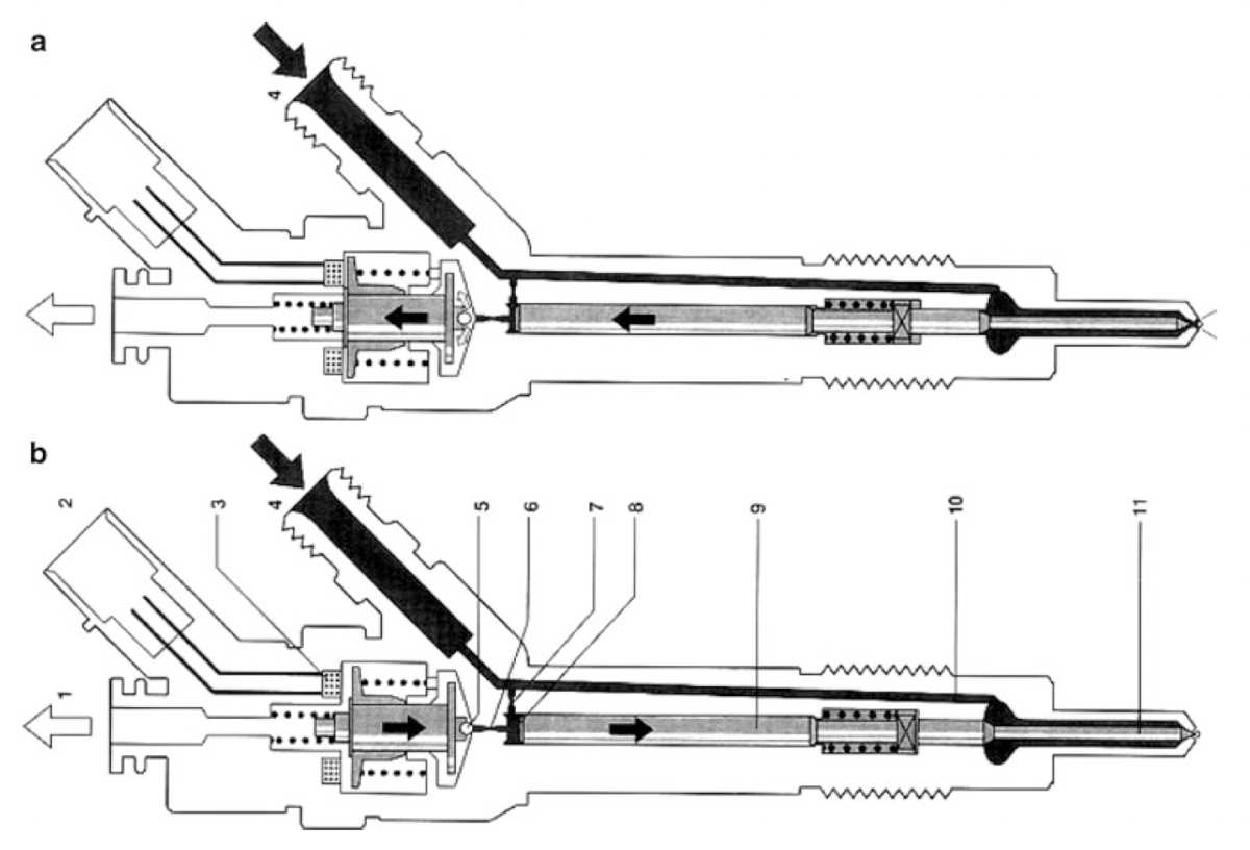
\includegraphics[width=0.7\textwidth]{images/EDC/EDC-6.pdf}
\caption{Injektors mit Magnetventil (bei Bosch bis zur Generation 2.16),
oben geöffnet, unten geschlossen. 1 Kraftstoff-Rücklauf, 2 elektrischer
Anschluss, 3 Elektromagnet, 4 Kraftstoff-Zulauf, 5 Ventilkugel, 6
Ablaufdrossel, 7 Zulaufdrossel, 8 Steuerraum, 9 Druckkolben, 10
Kraftstoff, 11 Nadel. (Bild: Robert Bosch GmbH)}
%\label{fig:}%% anpassen
\end{figure}

\emph{Wirkungskette:} Injektor öffnen $\to$ Steuergerät $\to$
Bestromung des Elektromagneten $\to$ Anzug des Ankers $\to$ Anheben
der Nadel $\to$ Einspritzung

\newpage

\begin{figure}[!ht]% hier: !ht
\centering
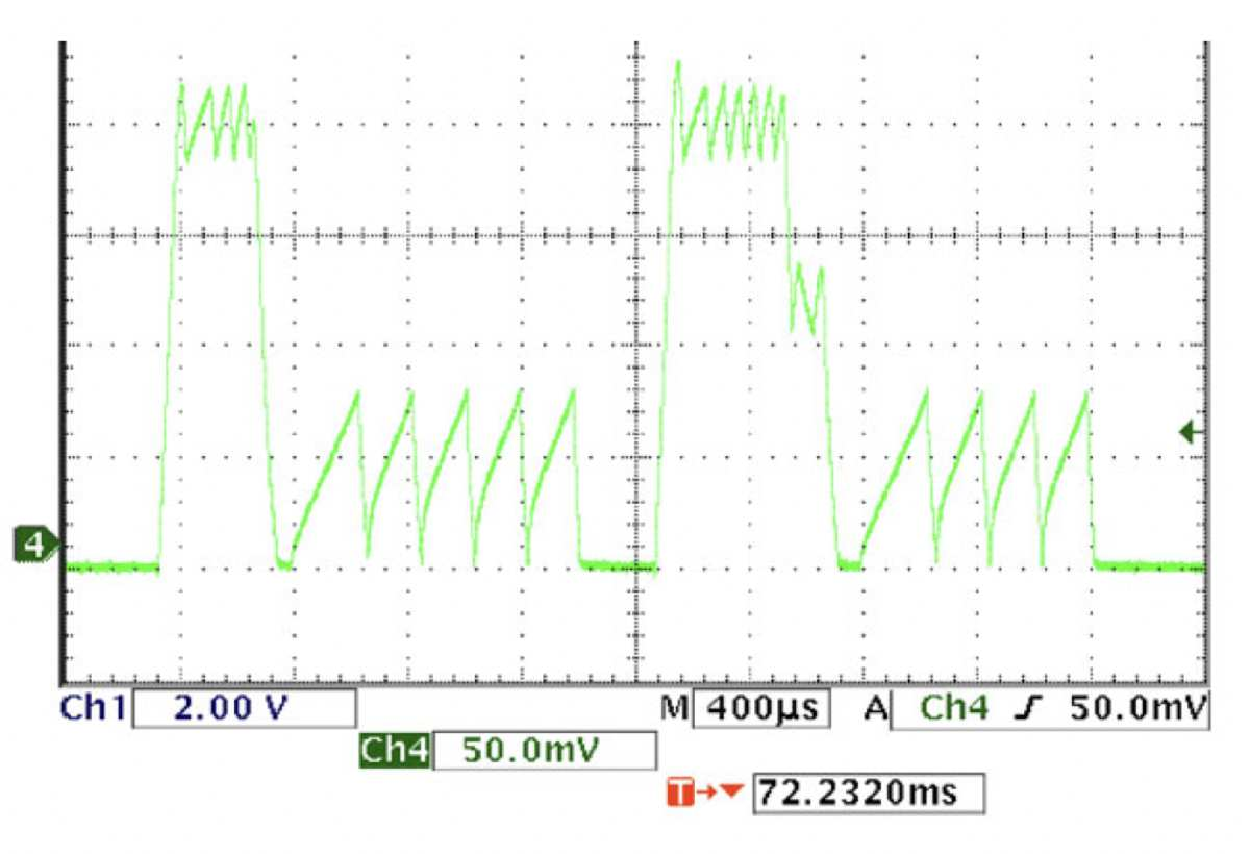
\includegraphics[width=0.5\textwidth]{images/EDC/EDC-7.pdf}
\caption{Zeitlicher Verlauf des Stromes durch einen Common-Rail-Injektor
bei einer Voreinspritzung und einer Haupteinspritzung. 1 Skalenteilung
entspricht vertikal einem Strom von 5 A, horizontal einer Dauer von 400
$\mu s$. (Bild: Kai Borgeest)}
%\label{fig:}%% anpassen
\end{figure}

Das Problem liegt nun darin, möglichst schnell den vollen Strom zu
erreichen, um den Anker hochzureißen. Dies lässt sich wegen der
Leitungsinduktivitäten nicht mit Hilfe der Fahrzeug-Batterie
realisieren. Stattdessen wird ein hinreichend großer Kondensator, auch
Booster-Kondensator genannt, im Steuergerät auf eine Spannung in der
Größenordnung 70 -- 90 V aufgeladen, der die Energie für den Anzug
liefert.

\begin{itemize}
\item
  Das erste Stromniveau von ca. 20 A ist der \textbf{Anzugsstrom}, der
  möglichst schnell den Anker heben soll. Eine sehr kurze Einspritzung
  wie die Voreinspritzung kann bereits während dieser Anzugsphase wieder
  enden. Nach einer Dauer von etwa einer halben Millisekunde kann davon
  ausgegangen werden, dass der Anker angezogen ist.
\item
  Von nun an genügt ein kleinerer Strom von z.B. 13 A, der
  \textbf{Haltestrom}, um den Anker in dieser Position zu halten.
\item
  Der zackige Verlauf der Stromniveaus ist darauf zurückzuführen, dass
  der Strom durch Ein- und Ausschalten von Transistoren um den mittleren
  Wert geregelt wird.
\end{itemize}

\textbf{Piezo-Injektoren}

Deren Aktorelement besteht aus einer piezoelektrischen Keramik die sich
bei Anlegen der Spannung um einige $10~\mu m$ dehnt. Über einen
hydraulischen Übersetzter betätigt das Piezo-Element ein Servoventil,
welches das Öffnen der Nadel ermöglicht.

\textbf{Vorteil} gegenüber einem Magnetventil ist ein kürzerer Verzug
zwischen der elektrischen Ansteuerung und dem Beginn der Einspritzung.

Aus elektrischer Sicht verhält sich ein Piezo-Injektor nicht wie eine
Spule, sondern wie ein Kondensator, der zum Einspritzen aufgeladen und
zum Schließen wieder entladen wird.

\begin{figure}[!ht]% hier: !ht
\centering
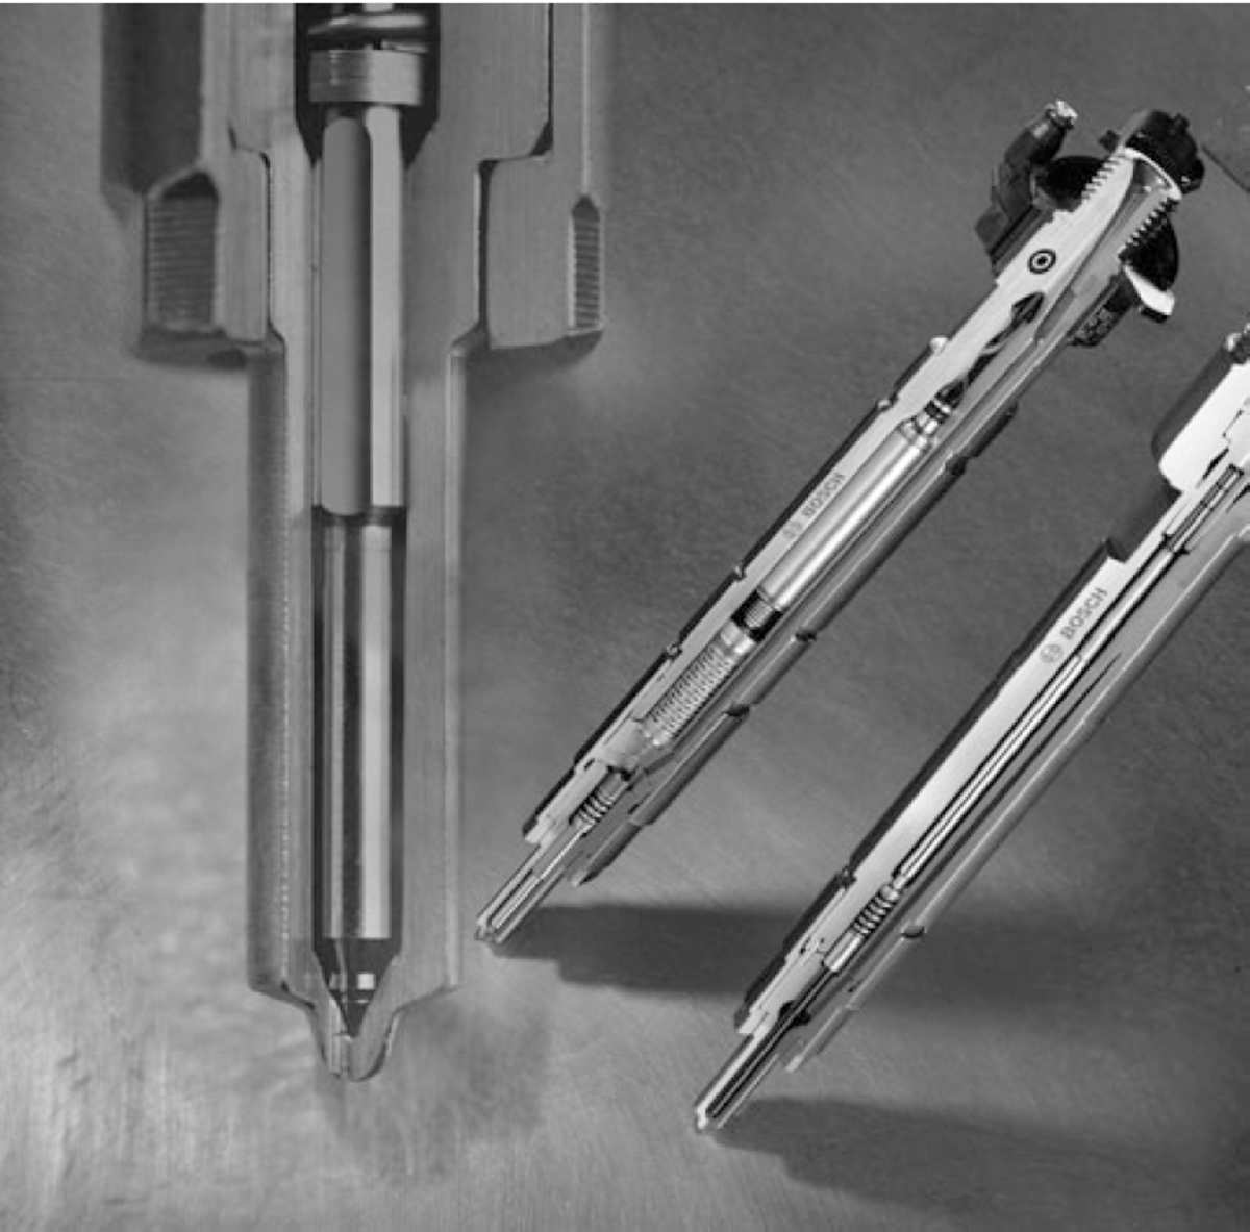
\includegraphics[width=0.5\textwidth]{images/EDC/EDC-9.pdf}
\caption{Vergleich zwischen Magnetventil-Injektor (rechts) und
Piezo-Injektor (Mitte). Links wird ein Detail einer Düsennadel gezeigt.
(Foto: Robert Bosch GmbH)}
%\label{fig:}%% anpassen
\end{figure}

\newpage

\subsection{Regelung des Raildrucks}\label{regelung-des-raildrucks}

\textbf{hoher Raildruck} ist wünschenswert, um eine feine Zerstäubung
des Kraftstoffs im Brennraum zu erreichen.

\textbf{Leerlauf} würde man mit einem maximalen Einspritzdruck von fast
3000 bar arbeiten, wäre der Motor unzumutbar laut und es wäre auch
schwierig, bei solchen hohen Drücken mit entsprechend kurzen
Ansteuerdauern kleine Mengen noch präzise darzustellen.

Man wird also zuerst abhängig vom Fahrzustand einen geeigneten Druck
auswählen und dann erst die Ansteuerdauer als Funktion der gewünschten
Menge und des Raildrucks berechnen.

\textbf{Raildrucksensoren} piezoresistive Sensoren, bei denen Änderungen
des Druckes in Änderungen des elektrischen Widerstandes umgesetzt
werden. Sie enthalten eine Metallmembran, die durch den Druck
durchgebogen wird. Auf dieser Membran sind vier Dehnungsmessstreifen so
aufgedampft oder mit Leitpaste aufgedruckt, dass zwei Streifen mit
zunehmender Biegung gestaucht, die anderen beiden gedehnt werden. Die
vier Streifen sind zu einer Wheatstone-Brücke verschaltet, in deren
Diagonalzweig eine zum Druck näherungsweise proportionale Spannung
abgegriffen werden kann. Heutige Sensoren enthalten bereits eine
Auswerteelektronik, welche die Brückenspannung auf die gewünschte
Ausgangsspannung umrechnet und Temperatureinflüsse kompensiert.

\newpage

\section{Drehzahlregelung}\label{drehzahlregelung}

\textbf{Änderung der Drehzahl} ergibt sich aus der

\begin{itemize}
\item
  Einspritzmenge, die wiederum vom Fahrerwunsch abhängt und
\item
  Last, die z. B. vom Fahrzeuggewicht und der Steigung abhängt.
\end{itemize}

\textbf{Sonderfall Leerlauf} wenn der Motor durch das Auskuppeln oder
weil kein Gang eingelegt ist, keinen Kraftschluss mit den Rädern hat und
der Fahrer kein Gas gibt, erwarten wir vom Motor einen ruhigen
gleichmäßigen Lauf ohne hörbare Drehzahlschwankungen.

\textbf{Leerlaufregler} benötigt zunächst eine Solldrehzahl.

\begin{itemize}
\item
  \textbf{zu hohe Leerlaufdrehzahl} würde den Kraftstoffverbrauch, die
  Lautstärke und die Emissionen von Schadstoffen erhöhen.
\item
  \textbf{zu niedrige Deerlaufdrehzahl} würde zu einem trägen
  Anfahrverhalten führen und der Generator könnte nicht mehr die
  benötigte Bordnetzspannung erzeugen.
\item
  Ein typischer Wert liegt bei $750~min^{-1}$.
\end{itemize}

\newpage

\section{Regelung des Luftsystems}\label{regelung-des-luftsystems}

\textbf{motorische Verbrennung} ist auf eine ausreichende Luftzufuhr
angewiesen. Reicht die Luft nicht aus, verbrennt der Kraftstoff
unvollständig. In Folge entstehen Schadstoffe und der Motor kann die
geforderte Leistung nicht bringen.

\textbf{Luftmangel erwünscht} der Verbrennungsprozess des Dieselmotors
ist mit höheren Spitzentemperaturen (zwischen $1000^\circ \text{C}$
und $2000^\circ \text{C}$) als bei Ottomotoren verbunden. Bei solch
hohen Temperaturen reagiert auch der in der Luft enthaltene Stickstoff
mit dem Sauerstoff. Es entstehen Stickoxide, vor allem Stickstoffmonoxid
(NO) und Stickstoffdioxid (NO2).

\textbf{Abgasrückführung (AGR) oder Exhaust Gas Recirculation (EGR)}
indem ein Teil des Abgases wieder zum Einlass des Zylinders rückgeführt
wird.

\textbf{Aufladen} um die Luftversorgung zu verbessern, saugt der Motor
nicht nur selbst Umgebungsluft an, sondern ein Turbolader pumpt
zusätzlich Luft in den Motor.

\newpage

\subsection{Abgasrückführung}\label{abgasrueckfuehrung}

\begin{itemize}
\item
  einen Teil der frischen Verbrennungsluft durch sauerstoffarmes Abgas
  zu ersetzen und damit die NOx-bildende Temperaturspitze bei der
  Verbrennung zu senken.
\item
  das hauptsächlich aus Wasser und Kohlendioxid bestehende Abgas eine
  höhere Wärmekapazität als Frischluft hat und so ebenfalls zur Senkung
  der Spitzentemperatur beiträgt.
\item
  Stickstoff, Sauerstoff, Kohlendioxid

  \begin{itemize}
  \item
    Stickstoff (N2) ist sowohl im Frischgas als auch im Restgas
    enthalten.
  \item
    Sauerstoff-Anteil (O2) ist im Abgas gegenüber dem Frischgas
    zumindest stark reduziert.
  \item
    Erhöht ist im Abgas der Anteil an Kohlendioxid (CO2) und Wasser
    (H2O) im gasförmigen Zustand.
  \end{itemize}
\item
  verschlechtert die Verbrennung künstlich und senkt so nicht nur den
  Stickoxid-Ausstoß, sondern auch die Motorleistung. Gleichzeitig
  entstehen mehr Rußpartikel durch die kältere Verbrennung.
\item
  Hochdruckrückführung und Niederdruckrückführung
\end{itemize}

\textbf{Abgasrückführrate} dient als Regelgröße. - Die maximal bei
PKW-Dieselmotoren eingesetzten Rückführraten liegen in der Größenordnung
um 50 \%, d.~h. die Hälfte der Zylinderfüllung stammt aus dem Abgas, der
Rest ist Frischluft. - Sobald die Rückführrate vom Sollwert abweicht, -
steigt entweder die \textbf{NOx-Emission} wieder drastisch an oder -
verbunden mit einem Leistungsverlust und einer Verkokung des Turboladers
die \textbf{Ruß-Emission}.

\begin{figure}[!ht]% hier: !ht
\centering
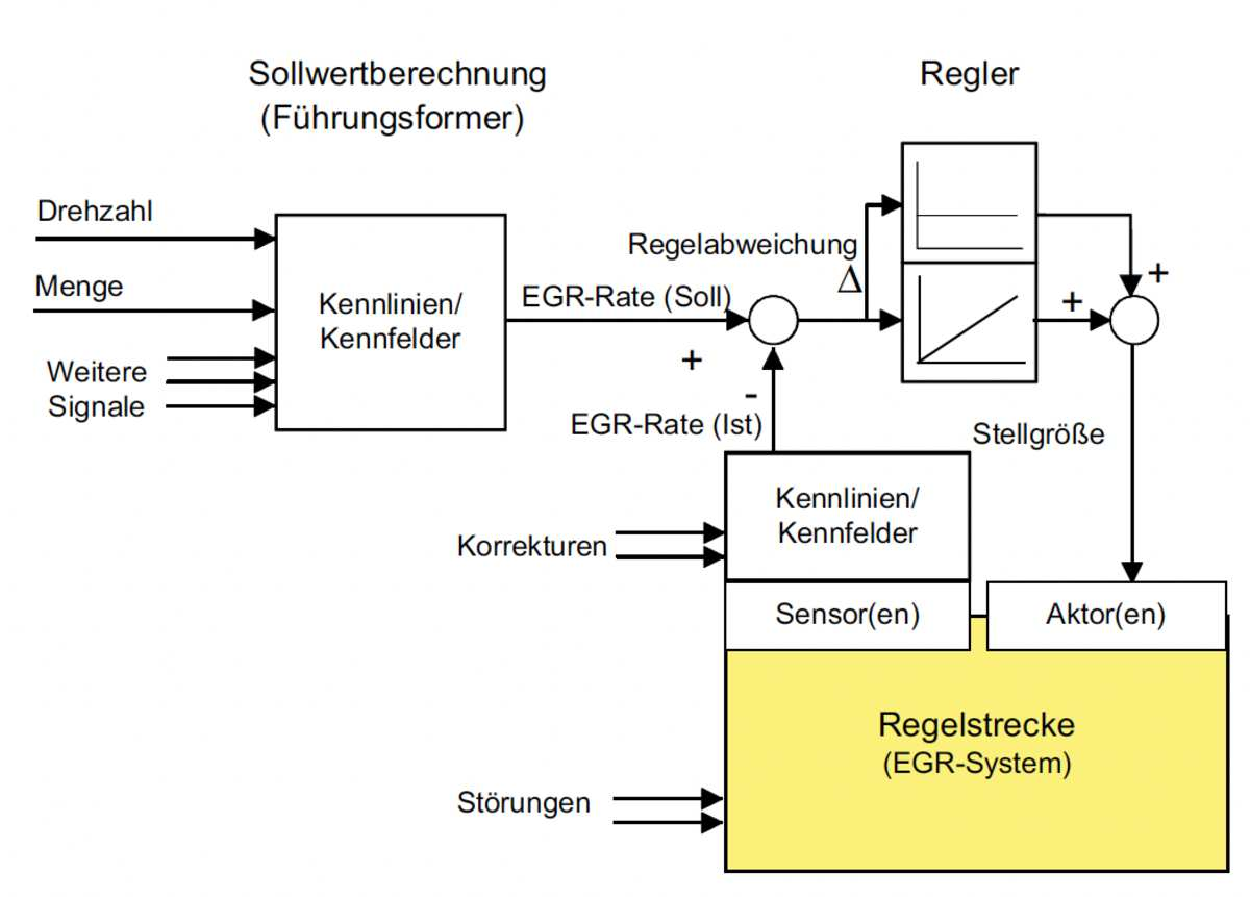
\includegraphics[width=0.5\textwidth]{images/EDC/EDC-10.pdf}
\caption{Regelung der Abgasrückführrate. (Bild: Kai Borgeest)}
%\label{fig:}%% anpassen
\end{figure}

\newpage

\subsection{Sensorik}\label{sensorik}

Luftmassenmesser (LMM), auch MAF (Mass Airflow Meter) misst die
angesaugte Frischluftmasse.

\begin{itemize}
\item
  Die \textbf{ältesten Luftmassenmesser} bestanden aus einer Klappe, die
  durch den Luftstrom angehoben wurde. Über ein Potenziometer konnte
  dann der Winkel dieser Klappe gemessen werden.
\item
  \textbf{Hitzdrahtsensoren}
\item
  \textbf{Heißfilm-Sensoren}

  \begin{itemize}
  \item
    in der Mitte des Sensorelements befindet sich eine beheizte Zone
    (4), auf beiden Seiten der Heizung befinden sich Temperatursensoren
    (M1 und M2).
  \item
    \emph{Wenn keine Luft} durch den Sensor strömt, stellt sich eine
    symmetrische Temperaturverteilung um die Heizung ein und beide
    Sensoren messen die gleiche Temperatur.
  \item
    \emph{Wenn nun Luft} (7) über die Oberfläche strömt, dann wird der
    in Strömungsrichtung vordere Sensor durch die Luft abgekühlt. Da die
    Luft über der Heizfläche Wärme aufnimmt, wird der hintere Sensor
    schwächer gekühlt.
  \item
    \emph{Temperaturdifferenz} vor und hinter der Heizfläche wird als
    Maß für die vorbeiströmende Luftmasse und auch für die
    Strömungsrichtung benutzt.
  \item
    Die vorbeiströmende Luft enthält Staub und Öldämpfe aus dem
    Kurbelgehäuse des Motors. Der Sensor muss trotzdem über die gesamte
    Fahrzeuglebensdauer präzise messen. Grobe Abweichungen können die
    Motorsteuergeräte über Plausibilitätsprüfungen selbst erkennen und
    als Defekt melden.
  \end{itemize}
\end{itemize}

\begin{figure}[!ht]% hier: !ht
\centering
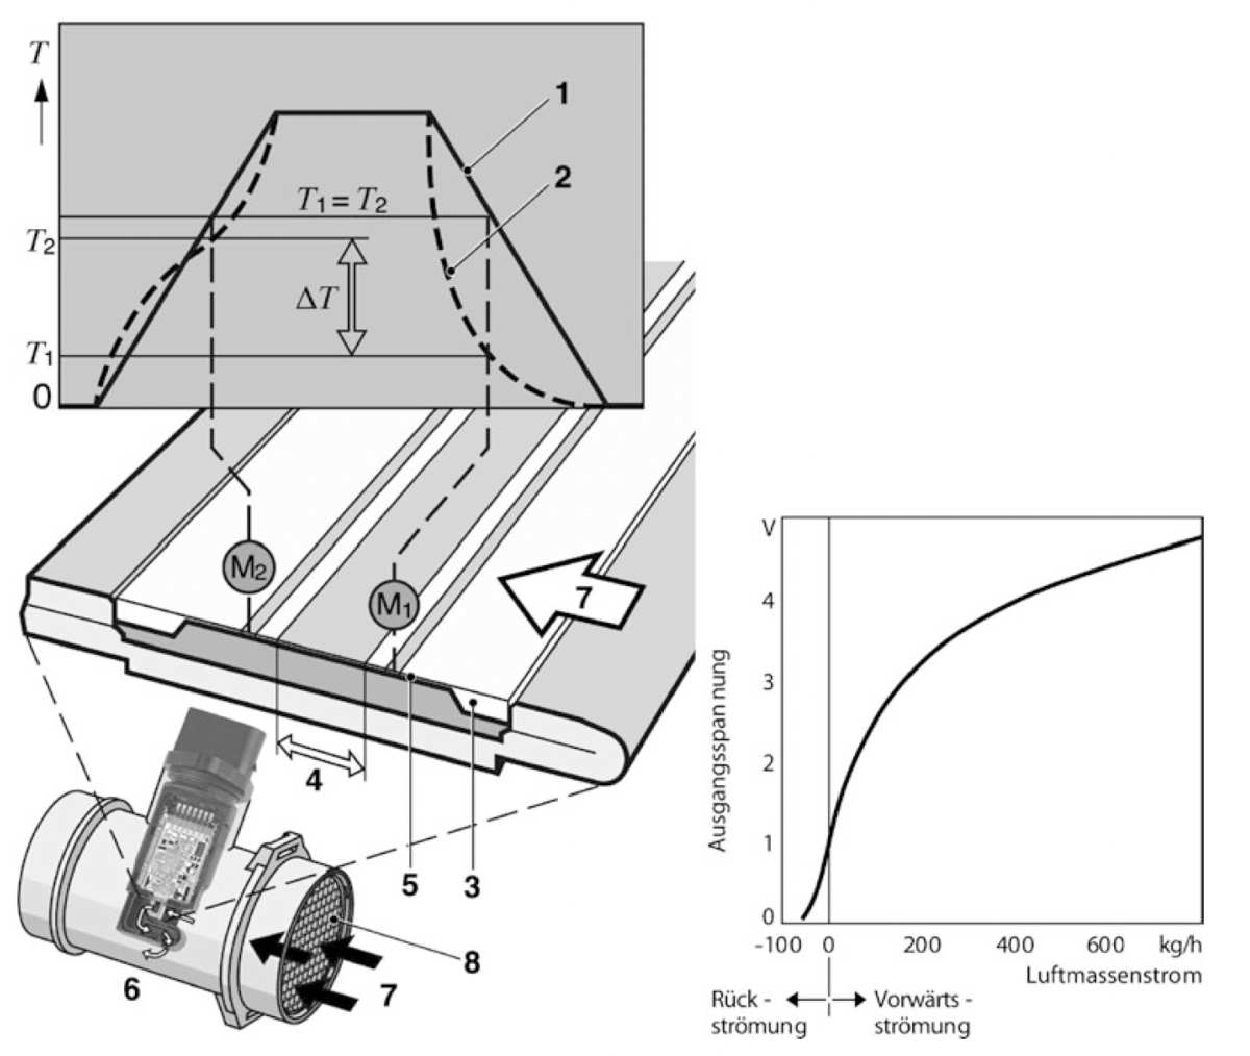
\includegraphics[width=0.5\textwidth]{images/EDC/EDC-11.pdf}
\caption{Aufbau und Prinzip des Heißfilm-Luftmassenmessers. (Bild:
Robert Bosch GmbH)}
%\label{fig:}%% anpassen
\end{figure}

\textbf{Lambda-Sonde} misst Restsauerstoff im Abgas

\newpage

\subsection{Aufladung}\label{aufladung}

Die \textbf{Luftmenge}, die ein Motor aufnehmen kann, wenn der Kolben im
Einlasstakt als saugende Pumpe wirkt, ist bei \textbf{Atmosphärendruck}
durch das Volumen des Zylinders begrenzt.

Erhöhen lässt sich die \textbf{Luftmenge}, wenn die Luft mit einem
\textbf{Überdruck} in den Zylinder gepresst wird. Dadurch verbrennt der
Kraftstoff in den Phasen, in denen eine große Menge eingespritzt wird,
besser und so entsteht weniger Rauch. Darüber hinaus lässt mit einer
größeren Luftfüllung auch mehr Kraftstoff verbrennen und mehr Leistung
erzeugen.

Tatsächlich lässt sich mit einer Verdopplung des Ladedrucks der gleiche
Effekt wie mit einer Verdopplung des Hubraums erzielen. Üblich sind
Ladedrücke bis zum 2,5-fachen Atmosphärendruck.

Ein \textbf{Turbolader} besteht aus einem Pumpenrad im Ansaugtrakt, das
über eine Welle von einer Turbine angetrieben wird. Die Turbine wird
durch die Energie im Abgasstrom angetrieben.

\begin{itemize}
\item
  \textbf{Vorteil} das die Abgasenergie sinnvoll genutzt wird und den
\item
  \textbf{Nachteil} das insbesondere bei kleinen Drehzahlen die Energie
  im Abgas nicht ausreicht, um einen nennenswert erhöhten Ladedruck
  aufzubauen. Dieser Drehzahlbereich wird umgangssprachlich auch als
  Turboloch bezeichnet und ist für den Fahrer spürbar.
\item
  \textbf{Aufgabe Motorsteuergerät} Ladedruck zu regeln und eine
  schädliche Drucküberhöhung zu vermeiden.

  \begin{itemize}
  \item
    Da der Ladedruck einen erheblichen Einfluss auf das Fahrverhalten
    und den Kraftstoffverbrauch hat, können Steuergeräte eventuell die
    Führungsgrößen passend zum messbaren Fahrstil auswählen. Selten wird
    die Abgastemperatur vor der Turbine gemessen, um den Turbolader vor
    Überhitzung schützen zu können.
  \end{itemize}
\end{itemize}

\newpage

\section{Abgasnachbehandlung
(Ergänzen)}\label{abgasnachbehandlung-ergaenzen}

\textbf{Maßnahmen zur Absenkung der Stickoxidemissionen}
Abgasrückführung oder späte Einspritzung erhöhen beim Dieselmotor die
Partikelemissionen.

\textbf{Maßnahmen zur Reduktion der Partikelemissionen} zu erhöhten
Emissionen von Stickoxiden.

\textbf{Möglichkeiten um schädliche Abgase zu minimieren}

\begin{enumerate}
\item
  ein Kompromiss zwischen Stickoxiden und Partikeln wird gesucht,
\item
  der Motor wird auf minimale NOx-Emissionen optimiert, die dabei
  zusätzlich entstehenden Partikel werden gefiltert,
\item
  der Motor wird auf minimale Partikelemissionen optimiert, die dabei
  zusätzlich entstehenden Stickoxide werden gefiltert oder
\item
  eine Abgasnachbehandlung reduziert zusätzlich NOx-Emissionen und
  Partikelemissionen.
\end{enumerate}

\begin{figure}[!ht]% hier: !ht
\centering
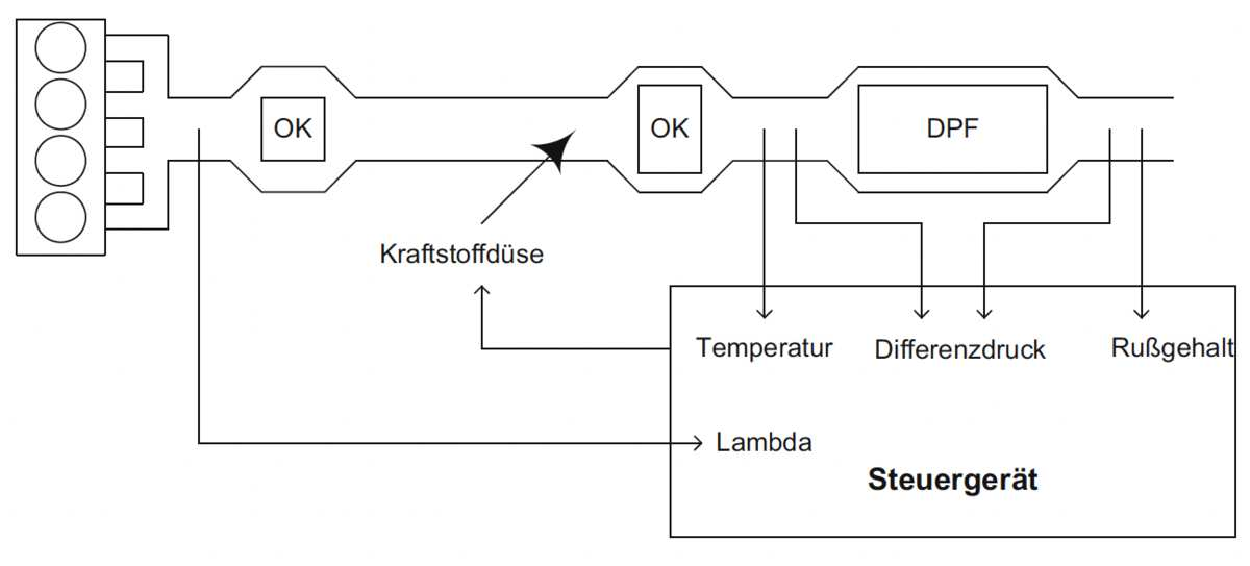
\includegraphics[width=0.5\textwidth]{images/EDC/EDC-13.pdf}
\caption{Umfangreich ausgestattetes Partikelfiltersystem mit zwei
Oxidationskatalysatoren (OK), Partikelfilter (DPF), Temperatur-,
Differenzdruck- und Rußsensor und zusätzlicher Kraftstoffeinspritzung in
den Abgastrakt. (Bild: Kai Borgeest)}
%\label{fig:}%% anpassen
\end{figure}

\begin{figure}[!ht]% hier: !ht
\centering
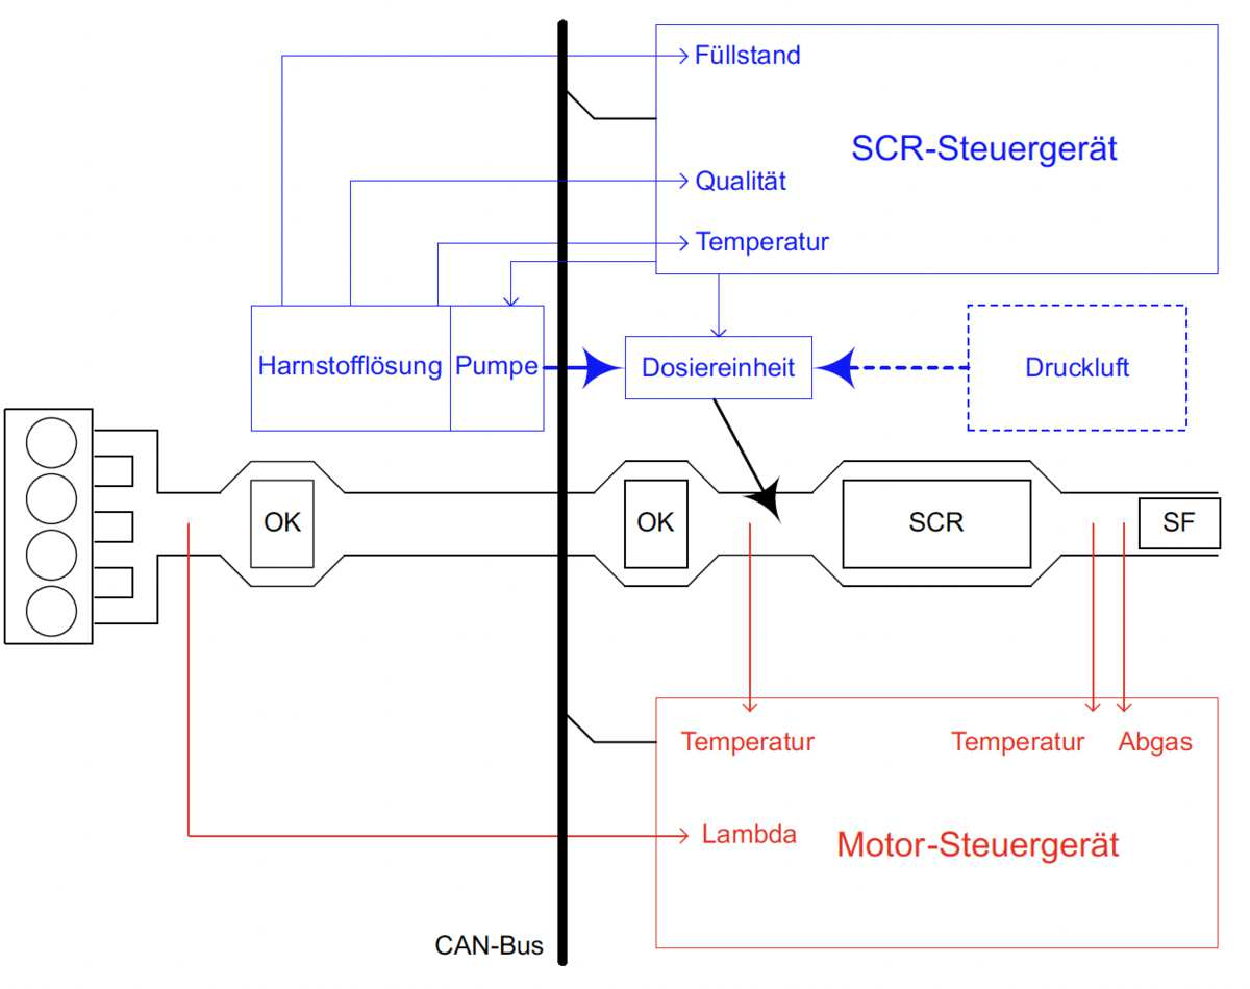
\includegraphics[width=0.5\textwidth]{images/EDC/EDC-14.pdf}
\caption{System zur selektiven katalytischen Reduktion (SCR) mit
Harnstoff-Einspritzung, Oxidations-Katalysatoren (OK) und einem
Ammoniak-Sperrfilter (SF). Da beide Steuergeräte über den CAN-Bus
kommunizieren, kann die Zuordnung der Sensoren zu den Steuergeräten auch
anders als im Bild erfolgen. (Bild: Kai Borgeest)}
%\label{fig:}%% anpassen
\end{figure}

\newpage

\section{Abgasskandal}\label{abgasskandal}

2015 wurde die Öffentlichkeit über die Medien informiert, dass
Automobilhersteller bei der Feststellung von Abgaswerten manipulierten,
um Fahrzeuge in den Markt zu bringen, die ohne Manipulationen nicht die
gesetzlichen Grenzwerte einhalten.

In der Vergangenheit wurde auf einem Rollenprüfstand ein genormter
Testzyklus (\textbf{NEFZ}, Neuer Europäischer Fahrzyklus) gefahren, die
Abgase während dieses Zyklus wurden gemessen und mit den gesetzlichen
Grenzwerten verglichen. Dieser Zyklus vermied emissionskritische
Situationen wie realistische Beschleunigungen und hohe
Geschwindigkeiten, außerdem enthielt er hohe Stillstandsanteile.

Der \textbf{Kern des Abgasskandals} lag nicht in der Verwendung eines
unrealistischen Zyklus, sondern darin, dass viele Fahrzeughersteller
Funktionen in der Software des Motorsteuergeräts oder des
Getriebesteuergeräts implementiert haben, die einen derartigen
Testzyklus von einer realen Straßenfahrt unterscheiden können.

Die bloße Erkennung ist \textbf{legal}, so muss z. B. das ABS
deaktiviert werden, wenn auf dem Rollenprüfstand nur die Antriebsräder
drehen, nicht hingegen die anderen Räder.

\textbf{Illegal} ist hingegen, das Verhalten des Motorsteuergerätes so
zu verändern, dass auf dem Prüfstand der Motor mit anderen Parametern
betrieben wird und damit faktisch im Straßenverkehr ein anderer Motor
als bei der Typprüfung eingesetzt wird (>>Cycle Beating<<). Auf dem
Prüfstand werden Abgasrückführung und Abgasnachbehandlung so geregelt,
dass die gesetzlichen Grenzwerte eingehalten werden, im Verkehr werden
diese Einrichtungen abgeschaltet oder vermindert eingesetzt.

Die \textbf{Unterscheidung zwischen Prüfstand und Straße} erfolgt über
die Auswertung von Fahrprofilen, der Umgebungsbedingungen (einige
Fahrzeuge reduzieren abgasreinigende Maßnahmen unterhalb
$17^\circ \text{C}$, weil für den NEFZ eine Mindesttemperatur von
$20^\circ \text{C}$ vorgeschrieben war) oder im einfachsten Fall über
einen Timer, der den Prüfstandsmodus nach Ablauf der Prüfzyklusdauer
abschaltet. Häufige illegale Eingriffe („Abschaltfunktionen>>) ins
Motormanagement sind z. B. unterschiedliche Abgasrückführraten oder
unterschiedliche SCR-Betriebsstrategien am Prüfstand und im
Straßenverkehr.

Für Neuzulassungen wurde 2017 in Europa ein realistischerer Testzyklus
im Rahmen der \textbf{WLTP} (Worldwide Harmonized Light Vehicles Test
Procedure) eingeführt, dieser wurde bereits vor etlichen Jahren
definiert, seine Einführung aber immer wieder verzögert.

Neu eingeführt wurde in der EU eine zusätzliche Straßenfahrt mit
Abgasmessung (Real Driving Emissions, \textbf{RDE}), eine Erkennung der
Abgasmessung wurde so erheblich erschwert.

\newpage

\section{Thermomanagement}\label{thermomanagement}

\textbf{Ziel} nach dem Start schnell die optimale Betriebstemperatur des
Motors von ca. $90^\circ \text{C}$ zu erreichen und dann zu halten.

\textbf{mechanisch angetriebene Wasserpumpe} und über eine
Zweipunktregelung mit Hilfe eines \textbf{Thermostaten}.

\begin{itemize}
\item
  Der Thermostat bewirkt, dass bei noch kaltem Motor das Kühlwasser
  zunächst nicht über den Luftwärmetauscher (Kühler) fließt, sondern nur
  in einem kleinen Kreislauf.
\end{itemize}

\textbf{elektrisch angetriebene Wasserpumpe}

\begin{itemize}
\item
  deren Verbreitung allerdings die hohe Leistung des Elektromotors
  entgegensteht. -
\item
  bei stehendem Motor z. B. um einen überhitzten Motor kontrolliert
  abzukühlen, ohne einen Temperaturschock des Motors zu riskieren.
\item
  Die erwähnte Kühlwassertemperatur von $90^\circ \text{C}$ beinhaltet
  einen großen \textbf{Sicherheitsspielraum}, weil die Flüssigkeit je
  nach Überdruck im Kühlsystem und chemischer Zusammensetzung erst bei
  etwa $110$ bis $120^\circ \text{C}$ zu sieden beginnt. Eine
  geregelte Wasserpumpe ermöglicht eine Verkleinerung des
  Sicherheitsspielraumes zugunsten des Motorwirkungsgrades.
\end{itemize}

\textbf{Thermosiphon-Kühlung} Motoren ohne Wasserpumpe, bei denen die
Konvektion (warmes Kühlmittel steigt aufgrund geringerer Dichte auf)
genügte, das Kühlwasser umzuwälzen. \textbf{Energieeinsparung} bei
schwacher Belastung des Motors die Wasserpumpe stillzulegen und zu
überbrücken, wenn der Kühlkreis so ausgelegt ist, dass durch Konvektion
eine ausreichende Kühlung sichergestellt ist.

\textbf{Gebläse mit einem Lüfterrad} hinter dem Kühler, das den
Luftstrom unterstützt, wenn der Fahrtwind nicht ausreicht.

\begin{itemize}
\item
  Das Gebläse wird vom Motorsteuergerät abhängig von der
  Kühlwassertemperatur gesteuert.
\item
  Eventuell wird es auch nach Abstellen des Fahrzeugs und Ausschalten
  der Zündung noch angesteuert. In diesem Falle muss das Steuergerät
  während des Lüfternachlaufs auch noch seine eigene Spannungsversorgung
  aufrechterhalten.
\item
  Bei größeren Motoren ist die \textbf{Leistung elektrischer Lüfter} zu
  hoch für das Bordnetz, in diesem Fall wird der Lüfter mechanisch über
  eine Ölkupplung (Visco-Kupplung) oder zukünftig evtl. über eine
  Kupplung aus Formgedächtnislegierungen angetrieben.
\end{itemize}

\textbf{elektrisch verstellbare Jalousie} vor dem Kühler, diese öffnet
bei hohem Kühlbedarf, ansonsten schließt sie ganz oder teilweise und
kann so auch die Aerodynamik des Fahrzeugs verbessern.

\textbf{elektrische Zuheizer} um schnell die Betriebstemperatur zu
erreichen, werden bereits heute bei Dieselmotoren mit hohem Wirkungsgrad
(und damit geringer Verlustleistung) im Kühlwasserkreislauf oder auch im
Ansauglufttrakt verwendet.

\begin{itemize}
\item
  \emph{PTC-Heizer} bei Erreichen einer Solltemperatur steigt deren
  Widerstand sprunghaft an und der Heizstrom sinkt.
\end{itemize}

\textbf{Ansteuerung der Glühkerzen} die Glühkerzen ragen bei >>direkt
einspritzenden Motoren<< in den Brennraum, bei >>Vorkammermotoren<<
heizen sie die Vorkammerwände auf.

\begin{itemize}
\item
  sollen eine schnellere Verdampfung des Kraftstoffes beim Kaltstart
  bewirken. Sie erreichen innerhalb weniger Sekunden
  Oberflächentemperaturen von über $1000^\circ \text{C}$.
\item
  lange Vorglühen eines Dieselmotors vor dem Start, einst
  umgangssprachlich als Diesel-Gedenkminute bezeichnet, ist mit heutigen
  Glühkerzen nur noch bei tiefem Frost nötig.
\item
  können einen Strom von über 30 A (pro Kerze, 4-Zylinder ca. 120 A)
  verbrauchen, dies zu einem Zeitpunkt, zu dem auch der Anlasser
  Leistung von der evtl. kälteschwachen Batterie abfordert und der
  Fahrer womöglich Großverbraucher wie die Heckscheibenheizung
  eingeschaltet hat.
\end{itemize}

\textbf{moderne Glühsysteme} bei denen die Kerzen nicht mehr über Relais
geschaltet werden, kann das Steuergerät die Spannung nach Erreichen der
Betriebstemperatur absenken und damit auch den Strom.

\begin{itemize}
\item
  \textbf{Zwischenglühen} können Glühkerzen zugeschaltet werden, um
  insbesondere im Leerlauf die Verbrennung und damit die Abgaswerte zu
  verbessern.
\item
  \textbf{gelbe Kontrollleuchte} wird im Armaturenbrett angesteuert. Um
  den Fahrer nicht zu irritieren, leuchtet sie nicht bei jedem
  Glühvorgang, sondern nur wenn es sinnvoll ist, mit dem Starten zu
  warten.
\end{itemize}

\textbf{Brennraumdruck-Sensoren} können in Glühkerzen integriert werden.


	%%%%%%%%%%%%%%%%%%%%%%%%%%%%%%%%%%%%%%%%%%%%%%%%%%%%%%%%%%%%%%%%%%
    % Bibliographie
    \printbibliography[category=cited]
\end{document}
